\chapter{无人机编队的动力学模型的建立}
\label{chap:formation_dynamic_equ}
本章基于无人机编队的领从方法(leader-follower method)建立无人机编队的相对运动方程。为了与无人机的解耦控制方法相匹配,本文的
模型建立将无人机运动分为水平平面运动以及竖直平面运动内分别建立数学模型。本文中采用北东地坐标系(NED)。领机与从机的各个运动学量分别
用下标$l,f$表示,领机、从机在三维空间内的运动量在图\ref{fig:c02-3d_rel_motion}表示;在水平以及竖直平面内的几何关系分别在图\ref{fig:c02-2d_level_motion}
和图\ref{fig:c02-2d_vert_motion}给出;
\begin{figure}
    \centering
    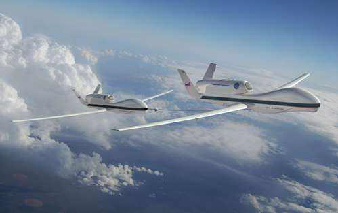
\includegraphics[width=0.5\textwidth]{figures/c01-meaning-1}
    \caption{三维空间双机编队几何关系}\label{fig:c02-3d_rel_motion}
\end{figure}
\begin{figure}
    \centering
    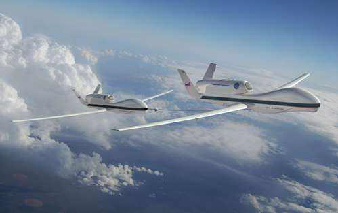
\includegraphics[width=0.5\textwidth]{figures/c01-meaning-1}
    \caption{水平平面双机编队几何关系}\label{fig:c02-2d_level_motion}
\end{figure}
\begin{figure}
    \centering
    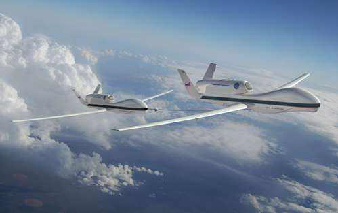
\includegraphics[width=0.5\textwidth]{figures/c01-meaning-1}
    \caption{竖直平面双机编队几何关系}\label{fig:c02-2d_vert_motion}
\end{figure}